\documentclass[a4paper]{article}
\usepackage[a4paper,margin=0mm]{geometry}
\usepackage{fontspec}
\usepackage{unicode-math}
\usepackage{tikz}
\usetikzlibrary{calc}
\usepackage[table]{xcolor}
\usepackage[absolute]{textpos}
\usepackage{enumitem}
\usepackage{array}
\usepackage{multirow}

\setmainfont{Libertinus Serif}
\setsansfont{Libertinus Sans}
\setmathfont{Libertinus Math}

\definecolor{accent}{HTML}{0F6A52}
\definecolor{badge}{HTML}{A9CFC2}
\definecolor{ink}{HTML}{2A2E30}

\setlength{\TPHorizModule}{1mm}
\setlength{\TPVertModule}{1mm}
\setlength{\parindent}{0pt}
\pagestyle{empty}
\binoppenalty=10000 \relpenalty=10000

\newcommand{\LCOL}{16mm}
\newcommand{\RCOL}{111mm}
\newcommand{\COLW}{83mm}

\newcommand{\topicheader}[2]{%
\begin{textblock*}{194mm}(16mm,10mm)
\begin{tikzpicture}
\node[fill=accent,text=white,font=\sffamily\bfseries\fontsize{13}{13}\selectfont,
      minimum width=9mm,minimum height=9mm,inner sep=0pt] at (4.5mm,-4.5mm) {#1};
\node[font=\sffamily\bfseries\fontsize{15}{16}\selectfont,text=ink,anchor=west] at (12mm,-4.5mm) {#2};
\end{tikzpicture}
\end{textblock*}
\begin{textblock*}{194mm}(16mm,22.5mm)

\begin{tikzpicture}
\fill[accent] (0,0) rectangle (194mm,0.5mm);
\end{tikzpicture}
\end{textblock*}
}

\newcommand{\pagefooter}[1]{%
\begin{textblock*}{194mm}(8mm,286.41mm)
  
\begin{tikzpicture}
    \fill[accent] (0,0) rectangle (194mm,0.6mm);
  \end{tikzpicture}
\end{textblock*}
\begin{textblock*}{63.59mm}(8mm,288.27mm)
  {\sffamily\bfseries\color{accent}\fontsize{13}{16}\selectfont SAT 1200+}
\end{textblock*}
\begin{textblock*}{10mm}(188mm,288.27mm)
  \centering{\sffamily\color{accent}\fontsize{14}{16}\selectfont #1}
\end{textblock*}
}

\newcommand{\colrule}[2]{%
\begin{textblock*}{1mm}(105mm,#1mm)
\begin{tikzpicture}
\draw[black!65,line width=0.5pt] (0,0) -- (0,#2mm);
\end{tikzpicture}
\end{textblock*}
}

% Page kicker: left = module line, right = question range
\newcommand{\pagekicker}[2]{%
\begin{textblock*}{194mm}(16mm,25.2mm)
{\sffamily\bfseries\fontsize{10.5}{12}\selectfont\color{accent}#1}\hfill{\sffamily\fontsize{10}{12}\selectfont\color{black!70}#2}
\end{textblock*}
}

\setlength{\fboxsep}{1.4pt}
\setlength{\fboxrule}{0.5pt}
\newcommand{\pnum}[1]{\fcolorbox{ink}{white}{\sffamily\bfseries\fontsize{8}{8}\selectfont #1}~}

% centered display line inside a stem
\newcommand{\dsp}[1]{\par\vspace{1.4mm}\centerline{#1}\vspace{1.8mm}}

% student-produced response box
\newcommand{\gridbox}{%
\par\vspace{3mm}\noindent

\begin{tikzpicture}
\node[anchor=south west,font=\sffamily\bfseries\fontsize{7.5}{9}\selectfont,text=accent,inner sep=0pt] at (0,0.3mm) {STUDENT-PRODUCED RESPONSE};
\draw[ink,line width=0.7pt] (0,-9.5mm) rectangle (40mm,-0.8mm);
\node[anchor=west,font=\sffamily\fontsize{7.5}{9}\selectfont,text=black!55,inner sep=0pt] at (43mm,-5.2mm) {Write your answer in the box.};
\end{tikzpicture}\par}

\arrayrulecolor{accent}
\setlength{\arrayrulewidth}{0.7pt}
\renewcommand{\arraystretch}{1.35}

\newcommand{\figwrap}[1]{\par\vspace{2.5mm}\centerline{{\arrayrulecolor{ink}\setlength{\arrayrulewidth}{0.5pt}\renewcommand{\arraystretch}{1.3}#1}}\vspace{0.5mm}}

\begin{document}

% ================= PAGE 1: Mock Test 10 -- instructions + geometry reference sheet =================
\topicheader{10}{Mock Test 10}
\pagefooter{221}
\mbox{}%

\newcommand{\cardhead}[1]{{\sffamily\bfseries\color{accent}\fontsize{11.5}{14}\selectfont #1}\par\vspace{0.6mm}%
{\color{accent}\rule{\linewidth}{0.5pt}}\par\vspace{1.6mm}}
\newcommand{\bul}{\item[\textcolor{accent}{\rule[0.2mm]{1.5mm}{1.5mm}}]}

\begin{textblock*}{194mm}(16mm,28mm)
{\sffamily\bfseries\color{accent}\fontsize{26}{28}\selectfont Mock Test 10\par}
\vspace{1mm}
{\sffamily\color{ink}\fontsize{11}{14}\selectfont Full-length digital SAT Math practice \;\textperiodcentered\; 2 modules $\times$ 22 questions $\times$ 35 minutes\par}
\end{textblock*}

\begin{textblock*}{\COLW}(\LCOL,53mm)
{\fontsize{9.4}{12.2}\selectfont
\cardhead{How this test works}
\renewcommand{\arraystretch}{1.3}\setlength{\tabcolsep}{4pt}
\noindent\begin{tabular}{|>{\raggedright\arraybackslash}p{20mm}|>{\centering\arraybackslash}p{15mm}|>{\centering\arraybackslash}p{13mm}|>{\centering\arraybackslash}p{19mm}|}
\hline
\rowcolor{badge!55}\textbf{Module} & \textbf{Questions} & \textbf{Time} & \textbf{Calculator}\\\hline
Module 1 & 22 & 35 min & allowed\\\hline
Module 2 & 22 & 35 min & allowed\\\hline
\end{tabular}\par\vspace{2.2mm}
\begin{itemize}[leftmargin=5mm,itemsep=1.2mm,topsep=0mm,parsep=0mm]
\bul Time each module separately: 35 minutes, not a minute more. Rest for 5--10 minutes between the two modules.
\bul Use a calculator (the built-in Desmos graphing calculator or any approved calculator) on both modules.
\bul Module 1 is a standard mix of easy, medium and hard questions. Module 2 is the \emph{harder route} you reach by doing well on Module 1.
\bul Answer every question. There is no penalty for a wrong answer.
\bul Unless a problem says otherwise, all numbers are real, a function's domain is every real number for which it is defined, and figures are not necessarily drawn to scale.
\bul Do not look at any answers while you work. When you finish both modules, score yourself with the \textbf{Answer Sheets} section at the end of this book.
\end{itemize}
}
\end{textblock*}

\begin{textblock*}{\COLW}(\RCOL,53mm)
{\fontsize{9.4}{12.2}\selectfont
\cardhead{Student-produced responses (grid-ins)}
Some questions have no answer choices. Work out the answer and write it in the answer box (on the real test you type it in).
\begin{itemize}[leftmargin=5mm,itemsep=1.2mm,topsep=1.6mm,parsep=0mm]
\bul You may give an integer, a decimal, or a fraction. For one answer, $9/2$ and $4.5$ are both correct.
\bul Never enter a mixed number: write $7/2$ or $3.5$, not $3\,1/2$ (it would be read as $31/2$).
\bul Do not enter symbols or units such as \$, \%, or $\pi$. Enter the number only.
\bul An answer may use at most 5 characters (6 if it is negative), counting the slash and the decimal point.
\bul If an answer is a repeating decimal, enter it as a fraction such as $2/3$, or fill all the digits that fit: $0.6666$ or $0.6667$.
\bul If you find more than one correct answer, enter only one of them.
\end{itemize}
\vspace{1.2mm}
\noindent\fcolorbox{accent}{badge!25}{\parbox{\dimexpr\linewidth-2\fboxsep-2\fboxrule}{\centering\sffamily\fontsize{8.5}{11}\selectfont
\textbf{Example.} Answer $4\tfrac12$ \;$\rightarrow$\; enter \textbf{9/2} or \textbf{4.5}\par}}
\par\vspace{3mm}
\noindent{\sffamily\bfseries\color{accent}Pacing.}\ Q1--15: about 18 min. Q16--22: about 17 min. Keep the last 2--3 min for flagged questions and every blank grid-in (a blank is a guaranteed zero).
}
\end{textblock*}

% ---- Geometry reference sheet (full width card) ----
\begin{textblock*}{178mm}(16mm,156mm)
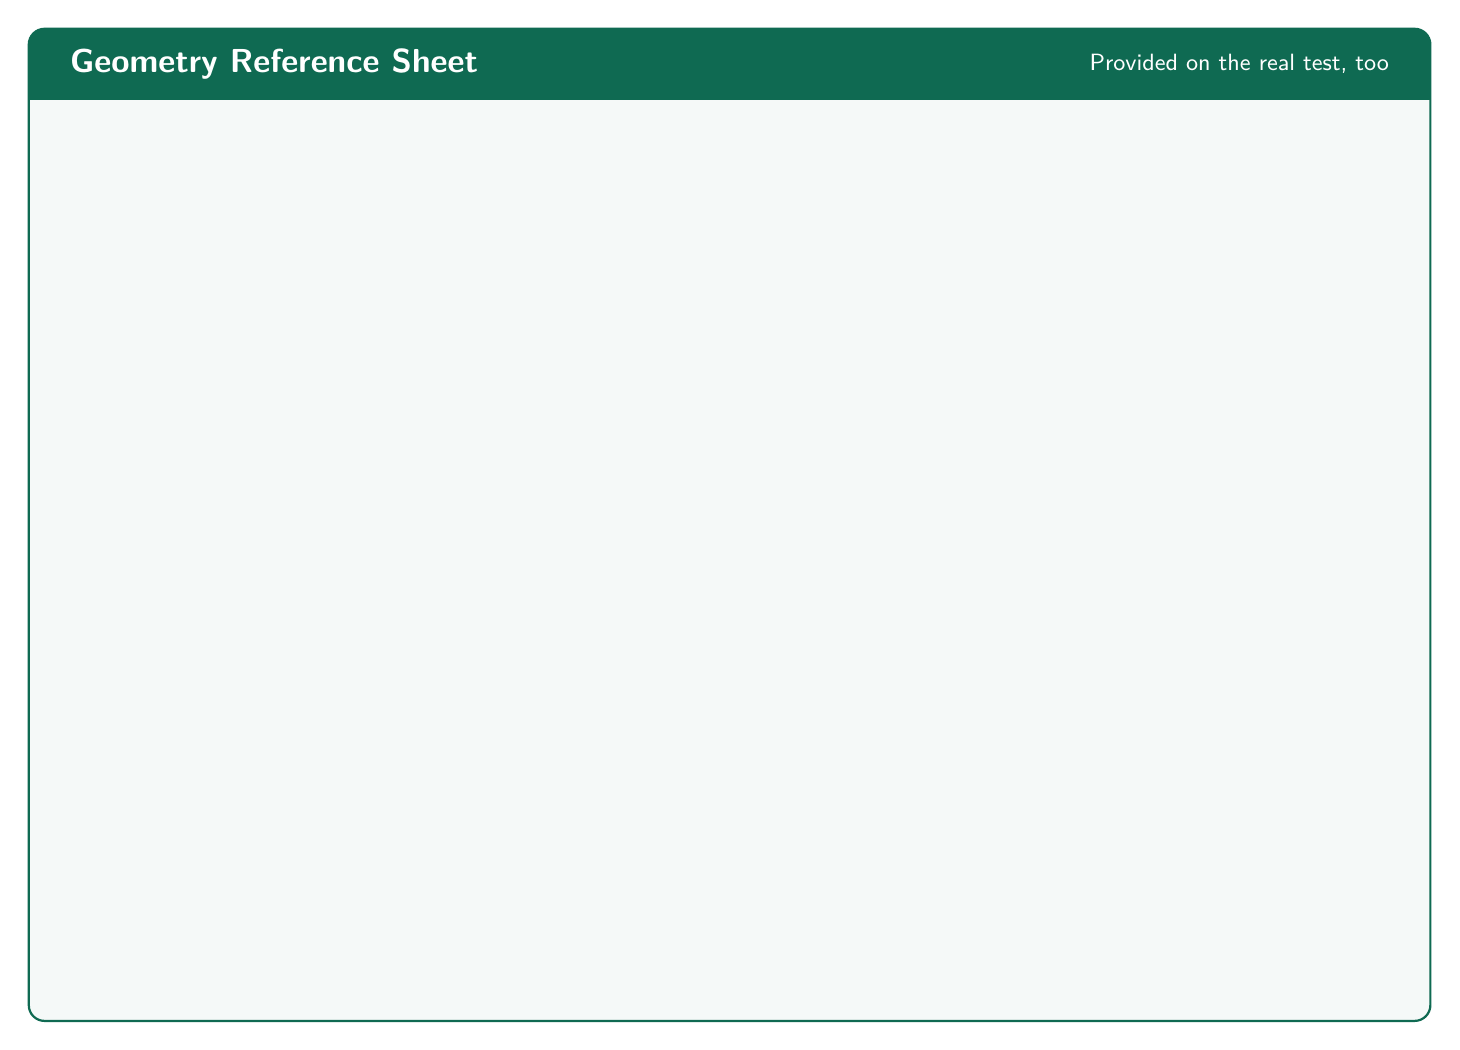
\begin{tikzpicture}
\draw[accent,line width=0.8pt,rounded corners=2mm,fill=badge!12] (0,0) rectangle (178mm,-126mm);
\fill[accent,rounded corners=2mm] (0,0) rectangle (178mm,-9mm);
\fill[accent] (0,-5mm) rectangle (178mm,-9mm);
\node[anchor=west,text=white,font=\sffamily\bfseries\fontsize{12}{14}\selectfont] at (4mm,-4.5mm) {Geometry Reference Sheet};
\node[anchor=east,text=white,font=\sffamily\fontsize{8.5}{10}\selectfont] at (174mm,-4.5mm) {Provided on the real test, too};
\end{tikzpicture}
\end{textblock*}

\newcommand{\refcell}[3]{\begin{textblock*}{42mm}(#1mm,#2mm)\begin{minipage}[t][36mm][t]{42mm}\centering #3\end{minipage}\end{textblock*}}
\newcommand{\refin}[2]{\parbox[b][26mm][b]{42mm}{\centering #1}\par\vspace{1.6mm}{\fontsize{9.6}{11.5}\selectfont #2}}
\tikzset{rf/.style={ink,line width=0.65pt},lb/.style={font=\fontsize{8.5}{9.5}\selectfont,inner sep=1.2pt}}

% ---------- row 1
\refcell{18}{167}{\refin{\begin{tikzpicture}[scale=1.25]
\draw[rf] (0,0) circle (9mm); \draw[rf] (0,0)--(9mm,0); \fill[ink] (0,0) circle (0.7pt);
\node[lb,above] at (4.5mm,0) {$r$};
\end{tikzpicture}}{Circle\\$A=\pi r^{2}$,\; $C=2\pi r$}}
\refcell{62}{167}{\refin{\begin{tikzpicture}[scale=1.25]
\draw[rf] (0,0) rectangle (22mm,12mm);
\node[lb,below] at (11mm,0) {$\ell$}; \node[lb,right] at (22mm,6mm) {$w$};
\end{tikzpicture}}{Rectangle\\$A=\ell w$}}
\refcell{106}{167}{\refin{\begin{tikzpicture}[scale=1.25]
\draw[rf] (0,0)--(22mm,0)--(7mm,13mm)--cycle;
\draw[rf,dashed] (7mm,0)--(7mm,13mm);
\draw[rf] (7mm,0)++(0,1.8mm)--++(1.8mm,0)--++(0,-1.8mm);
\node[lb,below] at (11mm,0) {$b$}; \node[lb,left] at (7mm,6.5mm) {$h$};
\end{tikzpicture}}{Triangle\\$A=\tfrac12 bh$}}
\refcell{150}{167}{\refin{\begin{tikzpicture}[scale=1.25]
\draw[rf] (0,0)--(18mm,0)--(0,12mm)--cycle;
\draw[rf] (0,1.8mm)--(1.8mm,1.8mm)--(1.8mm,0);
\node[lb,below] at (9mm,0) {$a$}; \node[lb,left] at (0,6mm) {$b$}; \node[lb,above right] at (9mm,6mm) {$c$};
\end{tikzpicture}}{Right triangle\\$c^{2}=a^{2}+b^{2}$}}

% ---------- row 2
\refcell{18}{204}{\refin{\begin{tikzpicture}[scale=1.25]
\draw[rf] (0,0)--(19.053mm,0)--(0,11mm)--cycle;
\draw[rf] (0,1.8mm)--(1.8mm,1.8mm)--(1.8mm,0);
\node[lb,below] at (9.5mm,0) {$x\sqrt3$}; \node[lb,left] at (0,5.5mm) {$x$}; \node[lb,above right] at (9.5mm,5.5mm) {$2x$};
\node[lb] at (14.6mm,1.9mm) {\fontsize{6.5}{7}\selectfont$30^\circ$}; \node[lb] at (3.2mm,8.2mm) {\fontsize{6.5}{7}\selectfont$60^\circ$};
\end{tikzpicture}}{$30^\circ$--$60^\circ$--$90^\circ$ triangle}}
\refcell{62}{204}{\refin{\begin{tikzpicture}[scale=1.25]
\draw[rf] (0,0)--(10mm,0)--(0,10mm)--cycle;
\draw[rf] (0,1.8mm)--(1.8mm,1.8mm)--(1.8mm,0);
\node[lb,below] at (5mm,0) {$s$}; \node[lb,left] at (0,5mm) {$s$}; \node[lb,above right] at (5mm,5mm) {$s\sqrt2$};
\end{tikzpicture}}{$45^\circ$--$45^\circ$--$90^\circ$ triangle}}
\refcell{106}{204}{\refin{\begin{tikzpicture}[scale=1.2]
\draw[rf] (0,0) rectangle (16mm,9mm);
\draw[rf] (16mm,9mm)--(22mm,13mm)--(6mm,13mm)--(0,9mm);
\draw[rf] (16mm,0)--(22mm,4mm)--(22mm,13mm);
\draw[rf,dashed] (6mm,13mm)--(6mm,4mm)--(22mm,4mm); \draw[rf,dashed] (0,0)--(6mm,4mm);
\node[lb,below] at (8mm,0) {$\ell$}; \node[lb,right] at (22mm,8.5mm) {$h$}; \node[lb,below right] at (19mm,2mm) {$w$};
\end{tikzpicture}}{Rectangular solid\\$V=\ell wh$}}
\refcell{150}{204}{\refin{\begin{tikzpicture}[scale=1.2]
\draw[rf] (0,2.2mm) ellipse (7mm and 2.2mm);
\draw[rf] (-7mm,2.2mm)--(-7mm,14mm); \draw[rf] (7mm,2.2mm)--(7mm,14mm);
\draw[rf] (0,14mm) ellipse (7mm and 2.2mm);
\draw[rf,dashed] (0,14mm)--(7mm,14mm); \fill[ink] (0,14mm) circle (0.6pt);
\node[lb,above] at (3.5mm,14mm) {$r$}; \node[lb,right] at (7mm,8mm) {$h$};
\end{tikzpicture}}{Right circular cylinder\\$V=\pi r^{2}h$}}

% ---------- row 3
\refcell{18}{241}{\refin{\begin{tikzpicture}[scale=1.15]
\draw[rf] (0,0) circle (10mm);
\draw[rf] (-10mm,0) arc (180:360:10mm and 2.8mm); \draw[rf,dashed] (-10mm,0) arc (180:0:10mm and 2.8mm);
\draw[rf] (0,0)--(10mm,0); \fill[ink] (0,0) circle (0.7pt); \node[lb,above] at (5mm,0) {$r$};
\end{tikzpicture}}{Sphere\\$V=\tfrac43\pi r^{3}$}}
\refcell{62}{241}{\refin{\begin{tikzpicture}[scale=1.2]
\draw[rf] (0,2.2mm) ellipse (7mm and 2.2mm);
\draw[rf] (-7mm,2.2mm)--(0,16mm)--(7mm,2.2mm);
\draw[rf,dashed] (0,16mm)--(0,2.2mm); \draw[rf,dashed] (0,2.2mm)--(7mm,2.2mm);
\fill[ink] (0,2.2mm) circle (0.6pt);
\node[lb,left] at (0,9.5mm) {$h$}; \node[lb,above] at (3.5mm,2.2mm) {$r$};
\end{tikzpicture}}{Right circular cone\\$V=\tfrac13\pi r^{2}h$}}
\refcell{106}{241}{\refin{\begin{tikzpicture}[scale=1.2]
\draw[rf] (0,0)--(16mm,0)--(22mm,4mm); \draw[rf] (0,0)--(10mm,15mm)--(16mm,0); \draw[rf] (10mm,15mm)--(22mm,4mm);
\draw[rf,dashed] (0,0)--(6mm,4mm)--(22mm,4mm); \draw[rf,dashed] (6mm,4mm)--(10mm,15mm);
\node[lb,below] at (8mm,0) {$\ell$}; \node[lb,below right] at (19mm,2mm) {$w$}; \node[lb,left] at (10mm,9.5mm) {$h$};
\end{tikzpicture}}{Rectangular pyramid\\$V=\tfrac13\ell wh$}}
\begin{textblock*}{40mm}(151mm,247mm)
{\fontsize{9.2}{12}\selectfont\raggedright
\textcolor{accent}{\rule[0.3mm]{1.6mm}{1.6mm}}\; A circle has 360 degrees of arc.\par\vspace{1.2mm}
\textcolor{accent}{\rule[0.3mm]{1.6mm}{1.6mm}}\; The angles of a triangle add up to 180 degrees.\par\vspace{1.2mm}
\textcolor{accent}{\rule[0.3mm]{1.6mm}{1.6mm}}\; $r$ radius, $\ell$ length, $w$ width, $b$ base, $h$ height.\par}
\end{textblock*}

\clearpage

% ===== Module 1, page 1 =====
\topicheader{10}{Mock Test 10}
\pagefooter{222}
\colrule{34}{236}
\mbox{}%
\pagekicker{Mock 10 \textperiodcentered{} Module 1 \textperiodcentered{} 22 questions \textperiodcentered{} 35 minutes}{Questions 1--8}
\begin{textblock*}{\COLW}(\LCOL,34mm)
{\fontsize{10.4}{13.4}\selectfont
\parbox[t][233mm][t]{\COLW}{%
\noindent\pnum{1} A trail runner starts a climb at an elevation of 1,200 feet and gains 400 feet of elevation each hour. After how many hours will the runner reach an elevation of 3,200 feet?\par\vspace{2.2mm}
\hspace*{7mm}(A)\ $8$\\[1.8mm]
\hspace*{7mm}(B)\ $11$\\[1.8mm]
\hspace*{7mm}(C)\ $5$\\[1.8mm]
\hspace*{7mm}(D)\ $2{,}000$
\vfill

\noindent\pnum{2} Which of the following is equivalent to $(3x^{4})^{2}$?\par\vspace{2.2mm}
\hspace*{7mm}(A)\ $9x^{8}$\\[1.8mm]
\hspace*{7mm}(B)\ $3x^{8}$\\[1.8mm]
\hspace*{7mm}(C)\ $9x^{6}$\\[1.8mm]
\hspace*{7mm}(D)\ $6x^{8}$
\vfill

\noindent\pnum{3} The lengths, in minutes, of six songs on a playlist are 3, 5, 4, 8, 6, and 4. What is the median length, in minutes, of the six songs?\gridbox
\vfill

\noindent\pnum{4} A cube-shaped planter has a volume of 343 cubic inches. What is the length, in inches, of one edge of the planter?\par\vspace{2.2mm}
\hspace*{7mm}(A)\ $\dfrac{343}{3}$\\[1.8mm]
\hspace*{7mm}(B)\ $49$\\[1.8mm]
\hspace*{7mm}(C)\ $14$\\[1.8mm]
\hspace*{7mm}(D)\ $7$
\vfill}}
\end{textblock*}
\begin{textblock*}{\COLW}(\RCOL,34mm)
{\fontsize{10.4}{13.4}\selectfont
\parbox[t][233mm][t]{\COLW}{%
\noindent\pnum{5} A charity needs 600 meal boxes packed. Volunteers have already packed 150 boxes and can pack 30 more boxes each hour. How many more hours will the volunteers need to reach 600 boxes?\par\vspace{2.2mm}
\hspace*{7mm}(A)\ $5$\\[1.8mm]
\hspace*{7mm}(B)\ $15$\\[1.8mm]
\hspace*{7mm}(C)\ $20$\\[1.8mm]
\hspace*{7mm}(D)\ $25$
\vfill

\noindent\pnum{6} The number of bacteria in a science-fair culture is modeled by $N(t)=40\cdot3^{t}$, where $t$ is the number of hours since the culture was started. According to the model, how many bacteria are in the culture at $t=2$?\par\vspace{2.2mm}
\hspace*{7mm}(A)\ $240$\\[1.8mm]
\hspace*{7mm}(B)\ $80$\\[1.8mm]
\hspace*{7mm}(C)\ $360$\\[1.8mm]
\hspace*{7mm}(D)\ $1{,}080$
\vfill

\noindent\pnum{7} A music streaming plan costs \$9 per month plus \$1.25 for each album downloaded that month. Lin's bill for one month was \$24. How many albums did she download that month?\gridbox
\vfill

\noindent\pnum{8} A city is building a wheelchair ramp that rises 0.9 meter over a horizontal distance of 1.2 meters. What is the length, in meters, of the sloped surface of the ramp?\par\vspace{2.2mm}
\hspace*{7mm}(A)\ $1.5$\\[1.8mm]
\hspace*{7mm}(B)\ $2.1$\\[1.8mm]
\hspace*{7mm}(C)\ $0.3$\\[1.8mm]
\hspace*{7mm}(D)\ $2.25$
\vfill}}
\end{textblock*}
\clearpage

% ===== Module 1, page 2 =====
\topicheader{10}{Mock Test 10}
\pagefooter{223}
\colrule{34}{236}
\mbox{}%
\pagekicker{Mock 10 \textperiodcentered{} Module 1 \textperiodcentered{} 22 questions \textperiodcentered{} 35 minutes}{Questions 9--16}
\begin{textblock*}{\COLW}(\LCOL,34mm)
{\fontsize{10.4}{13.4}\selectfont
\parbox[t][233mm][t]{\COLW}{%
\noindent\pnum{9} A science-fair team recorded the light exposure $x$, in minutes, and the height $y$, in millimeters, of 15 seedlings. The line of best fit is $y=6.4+0.38x$. One seedling had 50 minutes of exposure and a measured height of 27.1 millimeters. What is the residual for this seedling (measured height minus predicted height), in millimeters?\par\vspace{2.2mm}
\hspace*{7mm}(A)\ $25.4$\\[1.8mm]
\hspace*{7mm}(B)\ $-1.7$\\[1.8mm]
\hspace*{7mm}(C)\ $20.7$\\[1.8mm]
\hspace*{7mm}(D)\ $1.7$
\vfill

\noindent\pnum{10} A gardener has 18 square meters of bed space for tomatoes and peppers. Each square meter of tomatoes yields 9 kilograms, and each square meter of peppers yields 5 kilograms. All of the bed space is planted, and the total yield is 130 kilograms. How many square meters are planted with tomatoes?\gridbox
\vfill

\noindent\pnum{11} How many real solutions does the equation $\dfrac{x}{x-3}=2+\dfrac{3}{x-3}$ have?\par\vspace{2.2mm}
\hspace*{7mm}(A)\ $1$\\[1.8mm]
\hspace*{7mm}(B)\ $0$\\[1.8mm]
\hspace*{7mm}(C)\ $2$\\[1.8mm]
\hspace*{7mm}(D)\ $3$
\vfill

\noindent\pnum{12} The height, in meters, of a suspension-bridge cable above the deck is modeled by $h(x)=0.02x^{2}-1.2x+25$, where $x$ is the distance, in meters, from the left tower and $0\le x\le60$. What is the minimum height, in meters, of the cable above the deck?\par\vspace{2.2mm}
\hspace*{7mm}(A)\ $25$\\[1.8mm]
\hspace*{7mm}(B)\ $30$\\[1.8mm]
\hspace*{7mm}(C)\ $7$\\[1.8mm]
\hspace*{7mm}(D)\ $18$
\vfill}}
\end{textblock*}
\begin{textblock*}{\COLW}(\RCOL,34mm)
{\fontsize{10.4}{13.4}\selectfont
\parbox[t][233mm][t]{\COLW}{%
\noindent\pnum{13} A museum sells adult tickets for \$18 and child tickets for \$11. On one day the museum wants to collect at least \$900 and sell no more than 70 tickets in all. Which ordered pair $(a,c)$, where $a$ is the number of adult tickets and $c$ is the number of child tickets, satisfies both conditions?\par\vspace{2.2mm}
\hspace*{7mm}(A)\ $(30,35)$\\[1.8mm]
\hspace*{7mm}(B)\ $(20,40)$\\[1.8mm]
\hspace*{7mm}(C)\ $(45,35)$\\[1.8mm]
\hspace*{7mm}(D)\ $(25,30)$
\vfill

\noindent\pnum{14} If $2^{a}=3$ and $2^{b}=5$, what is the value of $2^{3a-b}$?\gridbox
\vfill

\noindent\pnum{15} The function $f$ is defined by $f(x)=x^{2}-8x+3$. If $f(a)=f(11)$ and $a\ne11$, what is the value of $a$?\par\vspace{2.2mm}
\hspace*{7mm}(A)\ $3$\\[1.8mm]
\hspace*{7mm}(B)\ $5$\\[1.8mm]
\hspace*{7mm}(C)\ $8$\\[1.8mm]
\hspace*{7mm}(D)\ $-3$
\vfill

\noindent\pnum{16} The table shows how 300 travelers booked a trip, by booking method and purpose of the trip. One traveler who booked on the website is chosen at random. What is the probability that the traveler's trip is for business?\figwrap{\begin{tabular}{|l|c|c|}
\hline
 & Business & Leisure\\\hline
App & 54 & 96\\\hline
Website & 66 & 48\\\hline
Travel agent & 18 & 18\\\hline
\end{tabular}}\par\vspace{2.2mm}
\hspace*{7mm}(A)\ $\dfrac{11}{50}$\\[1.8mm]
\hspace*{7mm}(B)\ $\dfrac{11}{19}$\\[1.8mm]
\hspace*{7mm}(C)\ $\dfrac{11}{23}$\\[1.8mm]
\hspace*{7mm}(D)\ $\dfrac{8}{19}$
\vfill}}
\end{textblock*}
\clearpage

% ===== Module 1, page 3 =====
\topicheader{10}{Mock Test 10}
\pagefooter{224}
\colrule{34}{236}
\mbox{}%
\pagekicker{Mock 10 \textperiodcentered{} Module 1 \textperiodcentered{} 22 questions \textperiodcentered{} 35 minutes}{Questions 17--22}
\begin{textblock*}{\COLW}(\LCOL,34mm)
{\fontsize{10.4}{13.4}\selectfont
\parbox[t][233mm][t]{\COLW}{%
\noindent\pnum{17} A travel site charges a fixed booking fee plus the same nightly rate for every night of a hotel stay. A 3-night stay costs \$472 and a 5-night stay costs \$748. What is the booking fee, in dollars?\gridbox
\vfill

\noindent\pnum{18} Which of the following is equivalent to $(3x-2)^{2}-(x+4)^{2}$?\par\vspace{2.2mm}
\hspace*{7mm}(A)\ $8x^{2}-12$\\[1.8mm]
\hspace*{7mm}(B)\ $8x^{2}-4x+20$\\[1.8mm]
\hspace*{7mm}(C)\ $8x^{2}-20x-12$\\[1.8mm]
\hspace*{7mm}(D)\ $4x^{2}-24x+36$
\vfill

\noindent\pnum{19} Maya is 4 years older than twice Leo's age. In 6 years, the sum of their ages will be 49. How old is Maya now?\par\vspace{2.2mm}
\hspace*{7mm}(A)\ $26$\\[1.8mm]
\hspace*{7mm}(B)\ $32$\\[1.8mm]
\hspace*{7mm}(C)\ $11$\\[1.8mm]
\hspace*{7mm}(D)\ $37$
\vfill}}
\end{textblock*}
\begin{textblock*}{\COLW}(\RCOL,34mm)
{\fontsize{10.4}{13.4}\selectfont
\parbox[t][233mm][t]{\COLW}{%
\noindent\pnum{20} What is the sum of all solutions of the equation $(x-4)^{2}=3(x-4)$?\par\vspace{2.2mm}
\hspace*{7mm}(A)\ $3$\\[1.8mm]
\hspace*{7mm}(B)\ $7$\\[1.8mm]
\hspace*{7mm}(C)\ $28$\\[1.8mm]
\hspace*{7mm}(D)\ $11$
\vfill

\noindent\pnum{21} The two distinct lines $2x+ky=10$ and $kx+8y=20$ in the $xy$-plane are parallel, where $k$ is a constant. What is the value of $k$?\gridbox
\vfill

\noindent\pnum{22} A regular hexagon is inscribed in a circle of radius 10, so all six vertices of the hexagon lie on the circle, as shown. What is the area of the region inside the circle and outside the hexagon?\figwrap{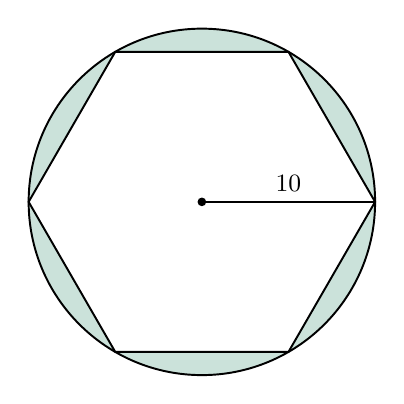
\begin{tikzpicture}[scale=0.22]
\fill[badge!60] (0,0) circle (10);
\fill[white] (10,0)--(5,8.660254)--(-5,8.660254)--(-10,0)--(-5,-8.660254)--(5,-8.660254)--cycle;
\draw[line width=0.7pt] (0,0) circle (10);
\draw[line width=0.7pt] (10,0)--(5,8.660254)--(-5,8.660254)--(-10,0)--(-5,-8.660254)--(5,-8.660254)--cycle;
\draw[line width=0.5pt] (0,0)--(10,0); \fill (0,0) circle (0.25);
\node[above,font=\small] at (5,0) {10};
\end{tikzpicture}}\par\vspace{2.2mm}
\hspace*{7mm}(A)\ $100\pi-100\sqrt{3}$\\[1.8mm]
\hspace*{7mm}(B)\ $100\pi-150\sqrt{3}$\\[1.8mm]
\hspace*{7mm}(C)\ $100\pi-75\sqrt{3}$\\[1.8mm]
\hspace*{7mm}(D)\ $100\pi-150$
\vfill}}
\end{textblock*}
\clearpage

% ===== Module 2, page 1 =====
\topicheader{10}{Mock Test 10}
\pagefooter{225}
\colrule{34}{236}
\mbox{}%
\pagekicker{Mock 10 \textperiodcentered{} Module 2 \textperiodcentered{} 22 questions \textperiodcentered{} 35 minutes}{Questions 1--8}
\begin{textblock*}{\COLW}(\LCOL,34mm)
{\fontsize{10.4}{13.4}\selectfont
\parbox[t][233mm][t]{\COLW}{%
\noindent\pnum{1} A booking site charges a \$40 service fee plus \$85 for each ticket. Marta's total was \$380. How many tickets did she buy?\par\vspace{2.2mm}
\hspace*{7mm}(A)\ $3$\\[1.8mm]
\hspace*{7mm}(B)\ $4$\\[1.8mm]
\hspace*{7mm}(C)\ $5$\\[1.8mm]
\hspace*{7mm}(D)\ $340$
\vfill

\noindent\pnum{2} The function $h$ is defined by $h(x)=3x^{2}-x+4$. What is the value of $h(-1)$?\par\vspace{2.2mm}
\hspace*{7mm}(A)\ $8$\\[1.8mm]
\hspace*{7mm}(B)\ $6$\\[1.8mm]
\hspace*{7mm}(C)\ $14$\\[1.8mm]
\hspace*{7mm}(D)\ $2$
\vfill

\noindent\pnum{3} A rectangular herb garden measures 20 feet by 14 feet. A walkway of uniform width $w$ feet surrounds the garden, and the walkway alone has an area of 152 square feet. What is the value of $w$?\par\vspace{2.2mm}
\hspace*{7mm}(A)\ $4$\\[1.8mm]
\hspace*{7mm}(B)\ $19$\\[1.8mm]
\hspace*{7mm}(C)\ $2$\\[1.8mm]
\hspace*{7mm}(D)\ $76$
\vfill

\noindent\pnum{4} A volunteer group assembles two kinds of kits for a shelter. Each type A kit holds 3 blankets and 2 bottles of water, and each type B kit holds 2 blankets and 5 bottles of water. The group uses exactly 62 blankets and exactly 100 bottles of water. How many kits did it assemble in all?\gridbox
\vfill}}
\end{textblock*}
\begin{textblock*}{\COLW}(\RCOL,34mm)
{\fontsize{10.4}{13.4}\selectfont
\parbox[t][233mm][t]{\COLW}{%
\noindent\pnum{5} A recording studio charges \$55 per hour for the first 10 hours of a booking and \$40 per hour for each additional hour. A band has a budget of \$1,000. What is the greatest whole number of hours the band can book?\par\vspace{2.2mm}
\hspace*{7mm}(A)\ $18$\\[1.8mm]
\hspace*{7mm}(B)\ $22$\\[1.8mm]
\hspace*{7mm}(C)\ $25$\\[1.8mm]
\hspace*{7mm}(D)\ $21$
\vfill

\noindent\pnum{6} A streaming service surveyed 40 subscribers about the number of playlists each one created last month. The table shows the results. How much greater is the median number of playlists than the mean number of playlists?\figwrap{\begin{tabular}{|l|c|c|c|c|c|}
\hline
Playlists created & 0 & 1 & 2 & 3 & 4\\\hline
Subscribers & 5 & 8 & 7 & 12 & 8\\\hline
\end{tabular}}\par\vspace{2.2mm}
\hspace*{7mm}(A)\ $0.5$\\[1.8mm]
\hspace*{7mm}(B)\ $0.25$\\[1.8mm]
\hspace*{7mm}(C)\ $0.75$\\[1.8mm]
\hspace*{7mm}(D)\ $2.5$
\vfill

\noindent\pnum{7} At 10:00 a.m. a hiker is at an elevation of 2,400 feet, and at 12:30 p.m. she is at 3,000 feet. She climbs at a constant rate the whole time, starting at the trailhead, which has an elevation of 1,800 feet. At what time did she start?\par\vspace{2.2mm}
\hspace*{7mm}(A)\ $7{:}30$ a.m.\\[1.8mm]
\hspace*{7mm}(B)\ $7{:}00$ a.m.\\[1.8mm]
\hspace*{7mm}(C)\ $8{:}00$ a.m.\\[1.8mm]
\hspace*{7mm}(D)\ $8{:}30$ a.m.
\vfill

\noindent\pnum{8} At a science fair, a team's profit, in dollars, from selling $x$ kits is $P(x)=-x^{2}+14x-24$, where $x$ is a whole number. For how many values of $x$ is the profit positive?\par\vspace{2.2mm}
\hspace*{7mm}(A)\ $13$\\[1.8mm]
\hspace*{7mm}(B)\ $11$\\[1.8mm]
\hspace*{7mm}(C)\ $9$\\[1.8mm]
\hspace*{7mm}(D)\ $10$
\vfill}}
\end{textblock*}
\clearpage

% ===== Module 2, page 2 =====
\topicheader{10}{Mock Test 10}
\pagefooter{226}
\colrule{34}{236}
\mbox{}%
\pagekicker{Mock 10 \textperiodcentered{} Module 2 \textperiodcentered{} 22 questions \textperiodcentered{} 35 minutes}{Questions 9--16}
\begin{textblock*}{\COLW}(\LCOL,34mm)
{\fontsize{10.4}{13.4}\selectfont
\parbox[t][233mm][t]{\COLW}{%
\noindent\pnum{9} Dana is 1.5 meters tall. She stands 6 meters from the base of a lamppost on level ground, and her shadow is 3 meters long. She then walks 4 meters directly away from the lamppost. How long, in meters, is her shadow now?\gridbox
\vfill

\noindent\pnum{10} A volunteer spends exactly \$100 on notebooks at \$7 each and pens at \$4 each, and she buys at least one of each item. In how many different ways can she make the purchase so that she buys more pens than notebooks?\par\vspace{2.2mm}
\hspace*{7mm}(A)\ $1$\\[1.8mm]
\hspace*{7mm}(B)\ $3$\\[1.8mm]
\hspace*{7mm}(C)\ $4$\\[1.8mm]
\hspace*{7mm}(D)\ $2$
\vfill

\noindent\pnum{11} A charity gala sells corporate tables for \$480 and individual tickets for \$45. The gala needs to collect at least \$6,000, and the hall holds at most 120 guests. Each table seats 8 guests and each individual ticket admits 1 guest. Which ordered pair $(t,i)$, where $t$ is the number of tables and $i$ is the number of individual tickets, satisfies both conditions?\par\vspace{2.2mm}
\hspace*{7mm}(A)\ $(6,60)$\\[1.8mm]
\hspace*{7mm}(B)\ $(12,30)$\\[1.8mm]
\hspace*{7mm}(C)\ $(10,30)$\\[1.8mm]
\hspace*{7mm}(D)\ $(8,40)$
\vfill

\noindent\pnum{12} The graph of $y=x^{2}-4x+1$ crosses the $x$-axis at $x=r$ and $x=s$. What is the value of $(r+3)(s+3)$?\par\vspace{2.2mm}
\hspace*{7mm}(A)\ $22$\\[1.8mm]
\hspace*{7mm}(B)\ $13$\\[1.8mm]
\hspace*{7mm}(C)\ $10$\\[1.8mm]
\hspace*{7mm}(D)\ $16$
\vfill}}
\end{textblock*}
\begin{textblock*}{\COLW}(\RCOL,34mm)
{\fontsize{10.4}{13.4}\selectfont
\parbox[t][233mm][t]{\COLW}{%
\noindent\pnum{13} The functions $f$ and $g$ are defined by $f(x)=x^{2}-6x+14$ and $g(x)=x^{2}-4x+1$. What is the minimum value of $g(f(x))$?\par\vspace{2.2mm}
\hspace*{7mm}(A)\ $-3$\\[1.8mm]
\hspace*{7mm}(B)\ $5$\\[1.8mm]
\hspace*{7mm}(C)\ $41$\\[1.8mm]
\hspace*{7mm}(D)\ $6$
\vfill

\noindent\pnum{14} A greenhouse harvests only tomatoes and peppers. From Year 1 to Year 2 the tomato harvest rose 20\%, the pepper harvest fell 10\%, and the total harvest rose 6\% to 1,590 kilograms. How many kilograms of peppers were harvested in Year 2?\par\vspace{2.2mm}
\hspace*{7mm}(A)\ $700$\\[1.8mm]
\hspace*{7mm}(B)\ $630$\\[1.8mm]
\hspace*{7mm}(C)\ $800$\\[1.8mm]
\hspace*{7mm}(D)\ $960$
\vfill

\noindent\pnum{15} A cubic polynomial $p$ satisfies $p(1)=p(3)=p(5)=7$ and $p(0)=-8$. What is the value of $p(6)$?\gridbox
\vfill

\noindent\pnum{16} Under a health plan, a patient whose bill $B$ is at least the deductible $d$ owes $P=d+r(B-d)$ dollars, where $r$ is the patient's share, as a decimal, of the amount above the deductible. A \$3,000 bill left a patient owing \$1,100, and a \$7,000 bill left a patient owing \$1,900. The plan also stops the patient's cost at \$2,000 per bill. What is the least bill, in dollars, for which the patient owes the full \$2,000?\par\vspace{2.2mm}
\hspace*{7mm}(A)\ $6{,}875$\\[1.8mm]
\hspace*{7mm}(B)\ $9{,}375$\\[1.8mm]
\hspace*{7mm}(C)\ $7{,}500$\\[1.8mm]
\hspace*{7mm}(D)\ $10{,}000$
\vfill}}
\end{textblock*}
\clearpage

% ===== Module 2, page 3 =====
\topicheader{10}{Mock Test 10}
\pagefooter{227}
\colrule{34}{236}
\mbox{}%
\pagekicker{Mock 10 \textperiodcentered{} Module 2 \textperiodcentered{} 22 questions \textperiodcentered{} 35 minutes}{Questions 17--22}
\begin{textblock*}{\COLW}(\LCOL,34mm)
{\fontsize{10.4}{13.4}\selectfont
\parbox[t][233mm][t]{\COLW}{%
\noindent\pnum{17} In right triangle $ABC$, the right angle is at $C$, the hypotenuse $AB$ has length 25, and the area of the triangle is 84. A circle with its center $P$ on $\overline{AB}$ is tangent to both $\overline{AC}$ and $\overline{BC}$, as shown. What is the radius of the circle?\figwrap{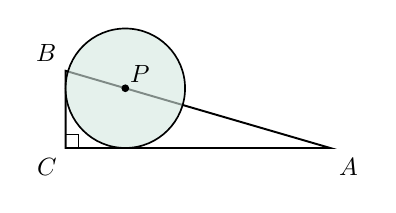
\begin{tikzpicture}[scale=0.14]
\draw[line width=0.7pt] (0,0)--(24,0)--(0,7)--cycle;
\draw[line width=0.5pt] (0,1.2)--(1.2,1.2)--(1.2,0);
\draw[line width=0.6pt,fill=badge!50,fill opacity=0.6] (5.419355,5.419355) circle (5.419355);
\fill (5.419355,5.419355) circle (0.35);
\node[below left,font=\small] at (0,0) {$C$};
\node[below right,font=\small] at (24,0) {$A$};
\node[above left,font=\small] at (0,7) {$B$};
\node[above right,font=\small,inner sep=1pt] at (5.6,5.6) {$P$};
\end{tikzpicture}}\par\vspace{2.2mm}
\hspace*{7mm}(A)\ $\dfrac{168}{31}$\\[1.8mm]
\hspace*{7mm}(B)\ $\dfrac{168}{25}$\\[1.8mm]
\hspace*{7mm}(C)\ $3$\\[1.8mm]
\hspace*{7mm}(D)\ $\dfrac{84}{31}$
\vfill

\noindent\pnum{18} A city surveyed residents about a proposed pedestrian plaza. Of the residents surveyed, 40\% commute by car, 35\% commute by transit, and 25\% commute by bike or on foot. Among car commuters, 30\% support the plaza, and among transit commuters, 60\% support it. A supporter of the plaza is selected at random, and the probability that this supporter commutes by car is $4/15$. What percent of the bike-or-foot commuters support the plaza? (Enter the number only.)\gridbox
\vfill

\noindent\pnum{19} What is the sum of all real solutions of the equation $|x^{2}-2x-8|=4x$?\par\vspace{2.2mm}
\hspace*{7mm}(A)\ $4$\\[1.8mm]
\hspace*{7mm}(B)\ $5+\sqrt{17}$\\[1.8mm]
\hspace*{7mm}(C)\ $1+\sqrt{17}$\\[1.8mm]
\hspace*{7mm}(D)\ $3+\sqrt{17}$
\vfill}}
\end{textblock*}
\begin{textblock*}{\COLW}(\RCOL,34mm)
{\fontsize{10.4}{13.4}\selectfont
\parbox[t][233mm][t]{\COLW}{%
\noindent\pnum{20} In the $xy$-plane, the graph of $x^{2}+y^{2}-10x+4y+k=0$, where $k$ is an integer, is a circle that intersects the $x$-axis at two points and does not intersect the $y$-axis at all. How many integer values of $k$ are possible?\par\vspace{2.2mm}
\hspace*{7mm}(A)\ $19$\\[1.8mm]
\hspace*{7mm}(B)\ $21$\\[1.8mm]
\hspace*{7mm}(C)\ $25$\\[1.8mm]
\hspace*{7mm}(D)\ $20$
\vfill

\noindent\pnum{21} For how many real values of $m$ does the system below have exactly one solution $(x,y)$ in the $xy$-plane?\dsp{$|x-3|=|y+2|$}\dsp{$y=mx-8$}\gridbox
\vfill

\noindent\pnum{22} In the $xy$-plane, the system below has exactly three distinct solutions $(x,y)$, where $k$ is a constant. What is the value of $k$?\dsp{$y=x^{2}-4$}\dsp{$x^{2}+y^{2}=k$}\par\vspace{2.2mm}
\hspace*{7mm}(A)\ $4$\\[1.8mm]
\hspace*{7mm}(B)\ $\dfrac{15}{4}$\\[1.8mm]
\hspace*{7mm}(C)\ $16$\\[1.8mm]
\hspace*{7mm}(D)\ $20$
\vfill}}
\end{textblock*}
\clearpage

\end{document}
